% vim: fo=aw2tq tw=100 spell
\chapter{Functional Overview}

\begin{nowordcount}
\begin{figure}[htbp]
\centering
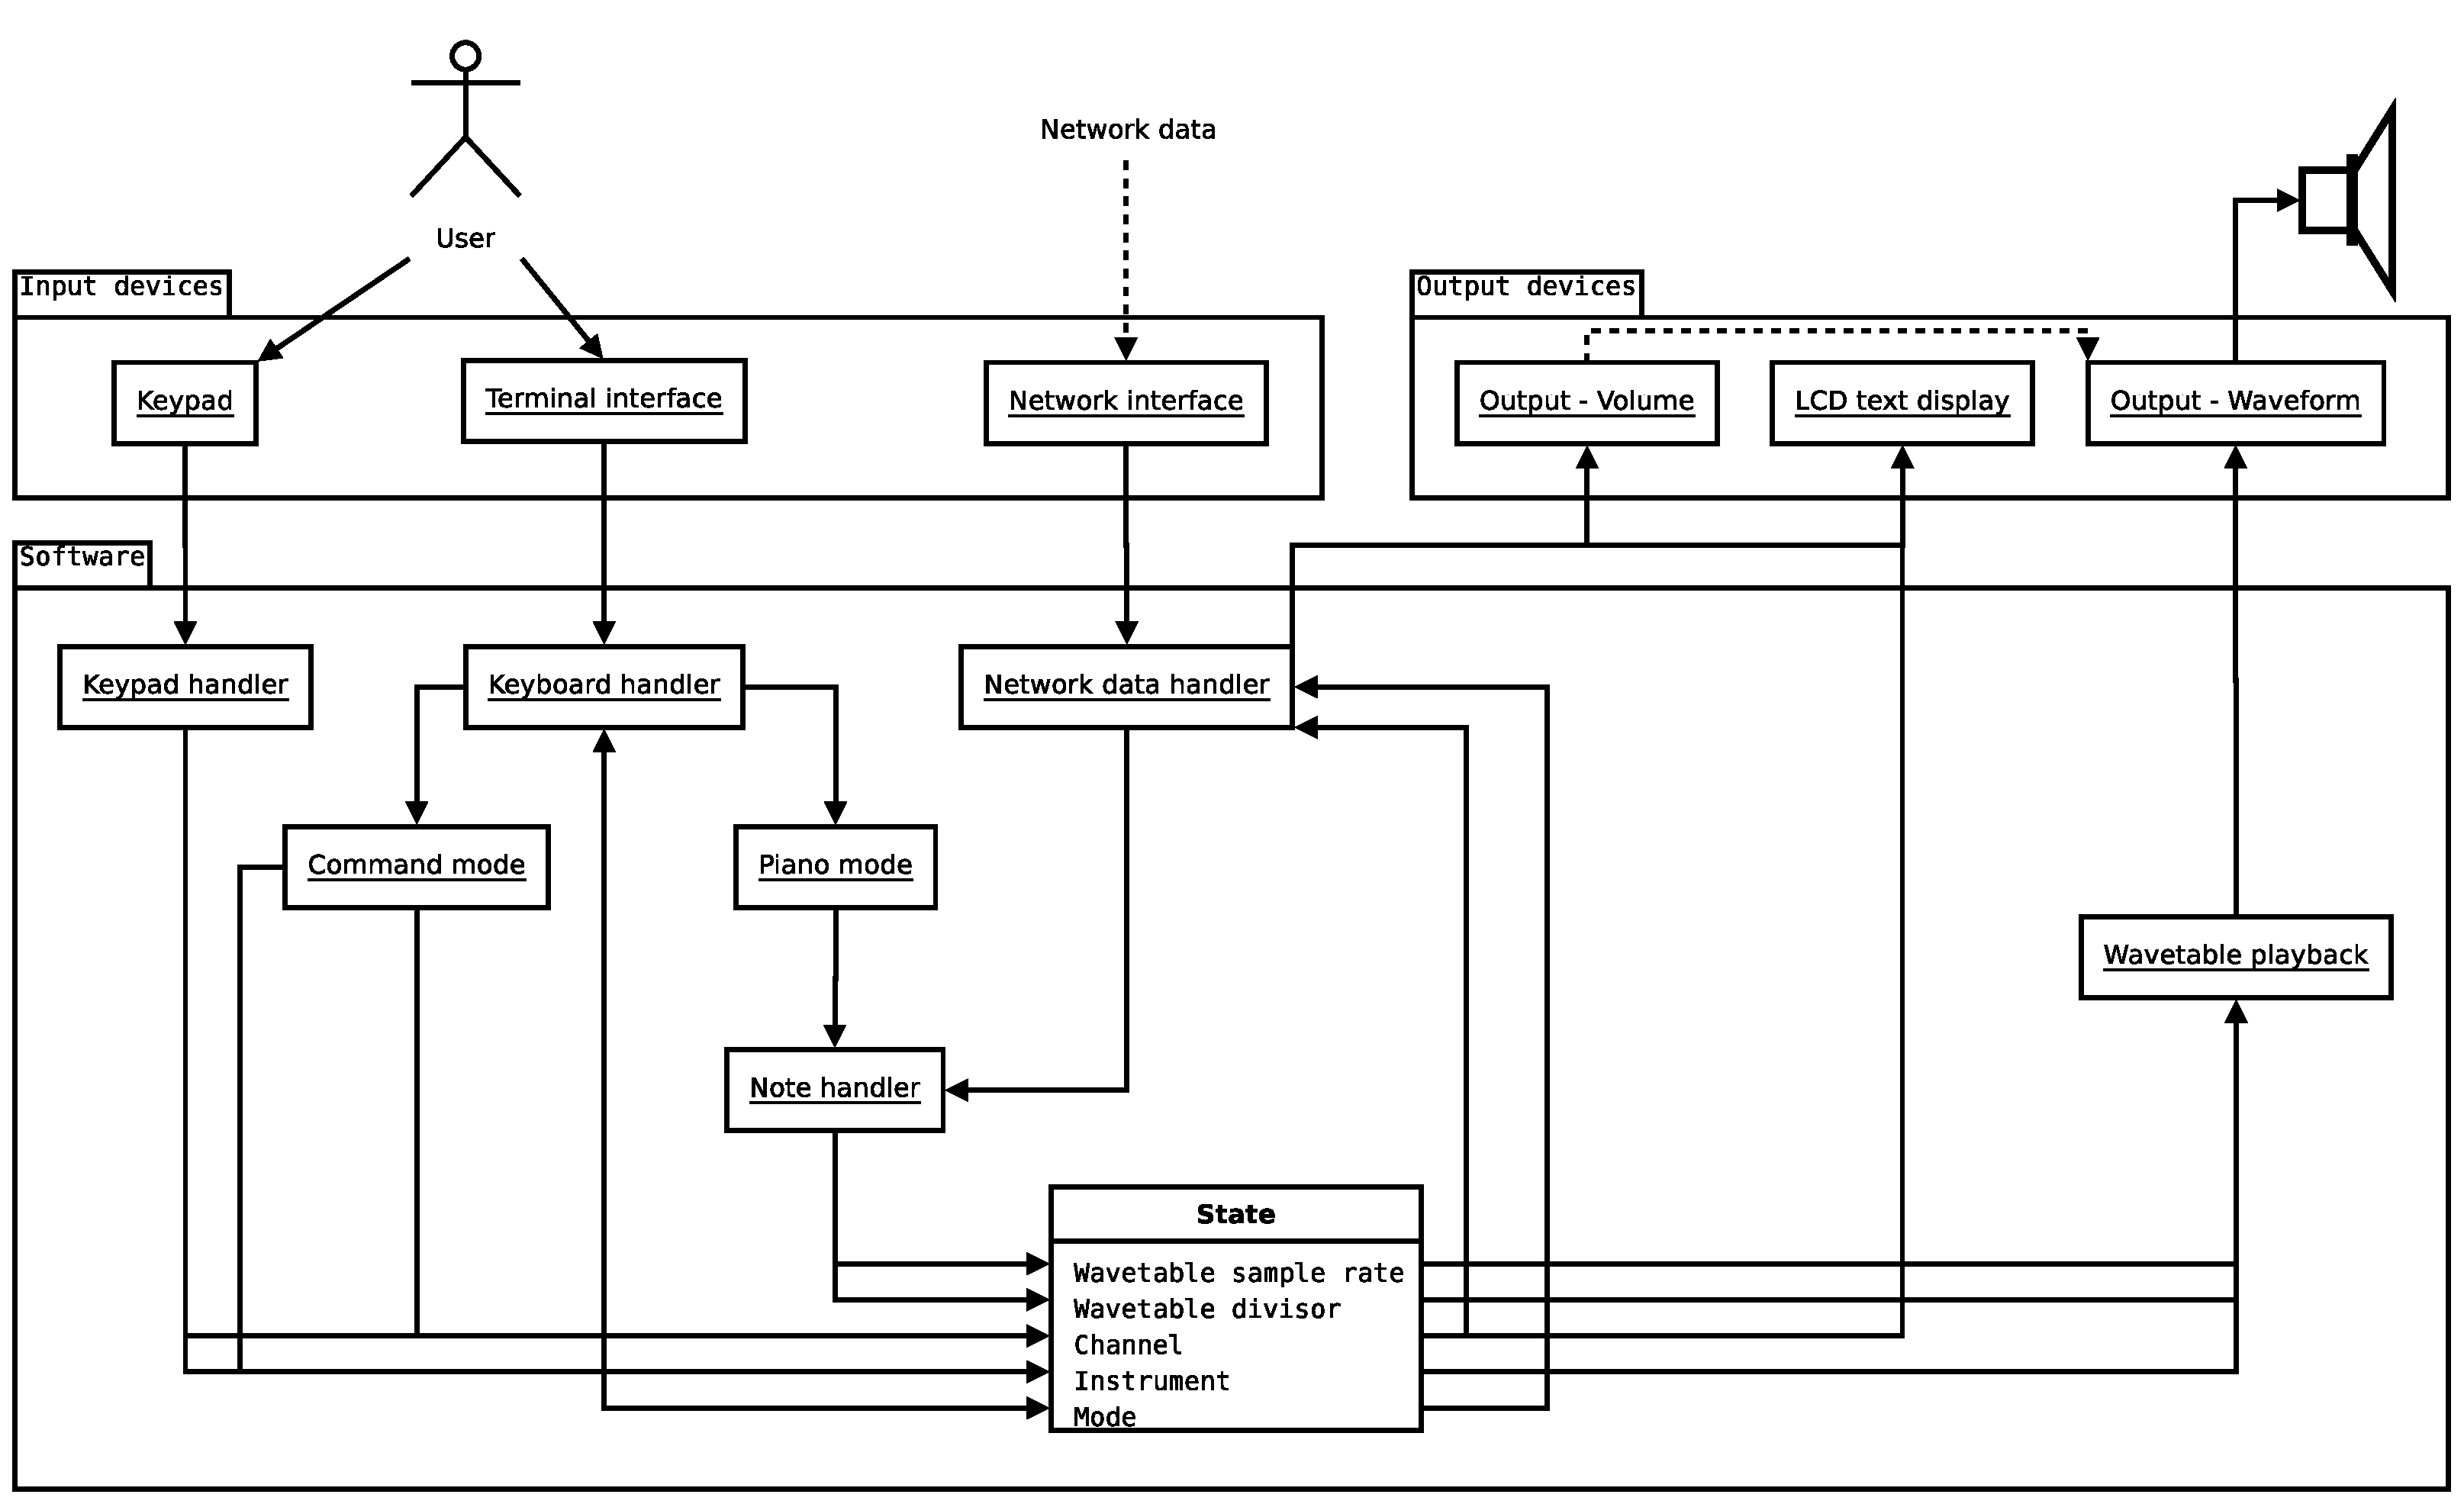
\includegraphics[totalheight=0.55\textheight,angle=90]{images/overview}
\caption{System Overview}\label{fig:systemoverview}
\end{figure}
\end{nowordcount}

The diagram in Figure \ref{fig:systemoverview} shows the conceptual architecture of my system.  The 
basic idea is that various inputs are processed and in some way modify the state of the system, and 
this state in turn affects the operation of the continuously-running wave table playback.

\section{Network Interface}
\label{sec:overview:network}

The network interface is a serial connection which receives a data stream at a rate of one 34-byte 
packet every $34ms$.  The data format is sixteen pairs of bytes, each pair containing a MIDI note 
value and a volume level (both in the range 0--127), with each pair representing a channel between 0 
and 15 (in order).  The packet is terminated with a null byte (00h) and a carriage return (0Dh).  
The mapping of channel identifiers to instruments is shown in Table \ref{tab:channelids}.  For the 
``Percussion'' channel, the volume level represents the particular percussion instrument to play 
rather than the volume at which to play it.

\begin{nowordcount}
\begin{table}[htbp]
\centering
\begin{tabular}{c | l}
ID & Instrument \\
\hline\hline
0 & Bass Guitar \\
1 & Cello \\
2 & Church Organ \\
3 & Piano \\
4 & Saxophone \\
5 & Melody \\
6 & Violin \\
7 & Trombone \\
8 & Trumpet \\
9 & French Horn \\
10 & Synth \\
11 & Electric Guitar \\
12 & Acoustic Guitar \\
13 & Flute \\
14 & Piccolo \\
15 & Percussion
\end{tabular}
\caption{Network data channels}\label{tab:channelids}
\end{table}
\end{nowordcount}

The network handler collects data from the incoming byte stream.  The bytes are counted, and the 
currently selected channel is used to decide which note/volume pair to store (see 
Section~\ref{sec:design:network-handler} for rationale on this design).  When the end of a packet is 
detected, the byte count is checked and the data discarded if the packet was incomplete.  The packet 
is also discarded if the system is not in ``network mode'' (see Section~\ref{sec:overview:state}).
If there is no reason to discard the packet, the data is used to set the state of the system.  The 
volume is converted to an 8-bit value (left-shifted) and output to the hardware, and also used to 
set the appropriate part of the LCD text display.  The note handler is run with the note value.

\section{Note Handler}
\label{sec:overview:note-handler}

The note handler ``receives'' a MIDI note value, and uses it to find the appropriate state 
information in a lookup tables.  Firstly, a playback lookup table is used to find the PRT value and 
divisor, which are written to the PRT reload register and divisor register used by the playback loop 
respectively.  Secondly, a display lookup table is used to find a 4-character representation of the 
note, which is written to the LCD text display.  See Section~\ref{sec:design:lookup-tables} for 
details of the lookup tables.

\section{Wavetable Playback}
\label{sec:overview:playback}

Wavetable playback is controlled by the PRT and divisor settings --- how these affect the frequency 
of the note is explained in Section~\ref{sec:design:wavetables}.  Every time the playback routine is 
called, the next sample from the wavetable for the current instrument is sent to the output device.  
The PRT reload value controls how often the playback routine is called.  The ``divisor'' controls 
the step between samples --- for example, 1 means every sample, 3 means every third sample.  The 
wavetable playback is affected only by the state of the system, it is not directly called from 
anywhere.

\section{Keypad Handler}
\label{sec:overview:keypad}

Since the keypad has 16 possible values, when a button is pressed on the keypad, the value is used 
to set the channel and instrument selection to that value.  \todo{Expand this.}

\section{Wave tables}
\label{wavetables}

\todo{Double check maths; move this to ``Design and Implementation''!}

In my design, all frequencies of the instruments are synthesised from the same wave table sample, 
therefore a way is needed to perform this frequency conversion.  A sample has two important 
interdependent properties --- the sample rate and the frequency.  When changing either of these 
properties, the following property holds:

\[\frac{F_{target}}{F_{source}} = \frac{R_{target}}{R_{source}}\]

In other words, if a particular note is recorded at a particular sample rate, then the difference of 
the frequency when played is proportional to the sample rate it is played at.  In this case, we are 
aiming to play a particular frequency, so the required sample rate can be calculated with:

\[R_{target} = \frac{F_{target} \times R_{source}}{F_{source}}\]

Unfortunately, at higher playback frequencies the necessary sample rate will be impractically high, 
so an additional way of changing the frequency is needed.  If for example only every other sample 
from the wave table is played, without changing the sample rate, this will double the frequency of 
the note being played, since the entire sample is being played twice as fast.  More generally, if a 
divisor $D$ is introduced, then $F_{target} = F_{source} \times D$.

To combine the two methods, $F_{target}$ can be replaced with $F_{target} \times D$.  With a little 
re-arrangement, the following equation can be obtained:

\[R_{target} \times D = \frac{F_{target} \times R_{source}}{F_{source}}\]

See \ref{notelookuptables} for how this conversion is implemented to generate the MIDI note lookup 
tables.
